% Teilauswertung 2
\newpage
\section{Dunkelfeldspektroskopie einer Nanorodprobe}
\label{sec:nanorods}

\begin{center}
    \captionsetup{type = figure}
    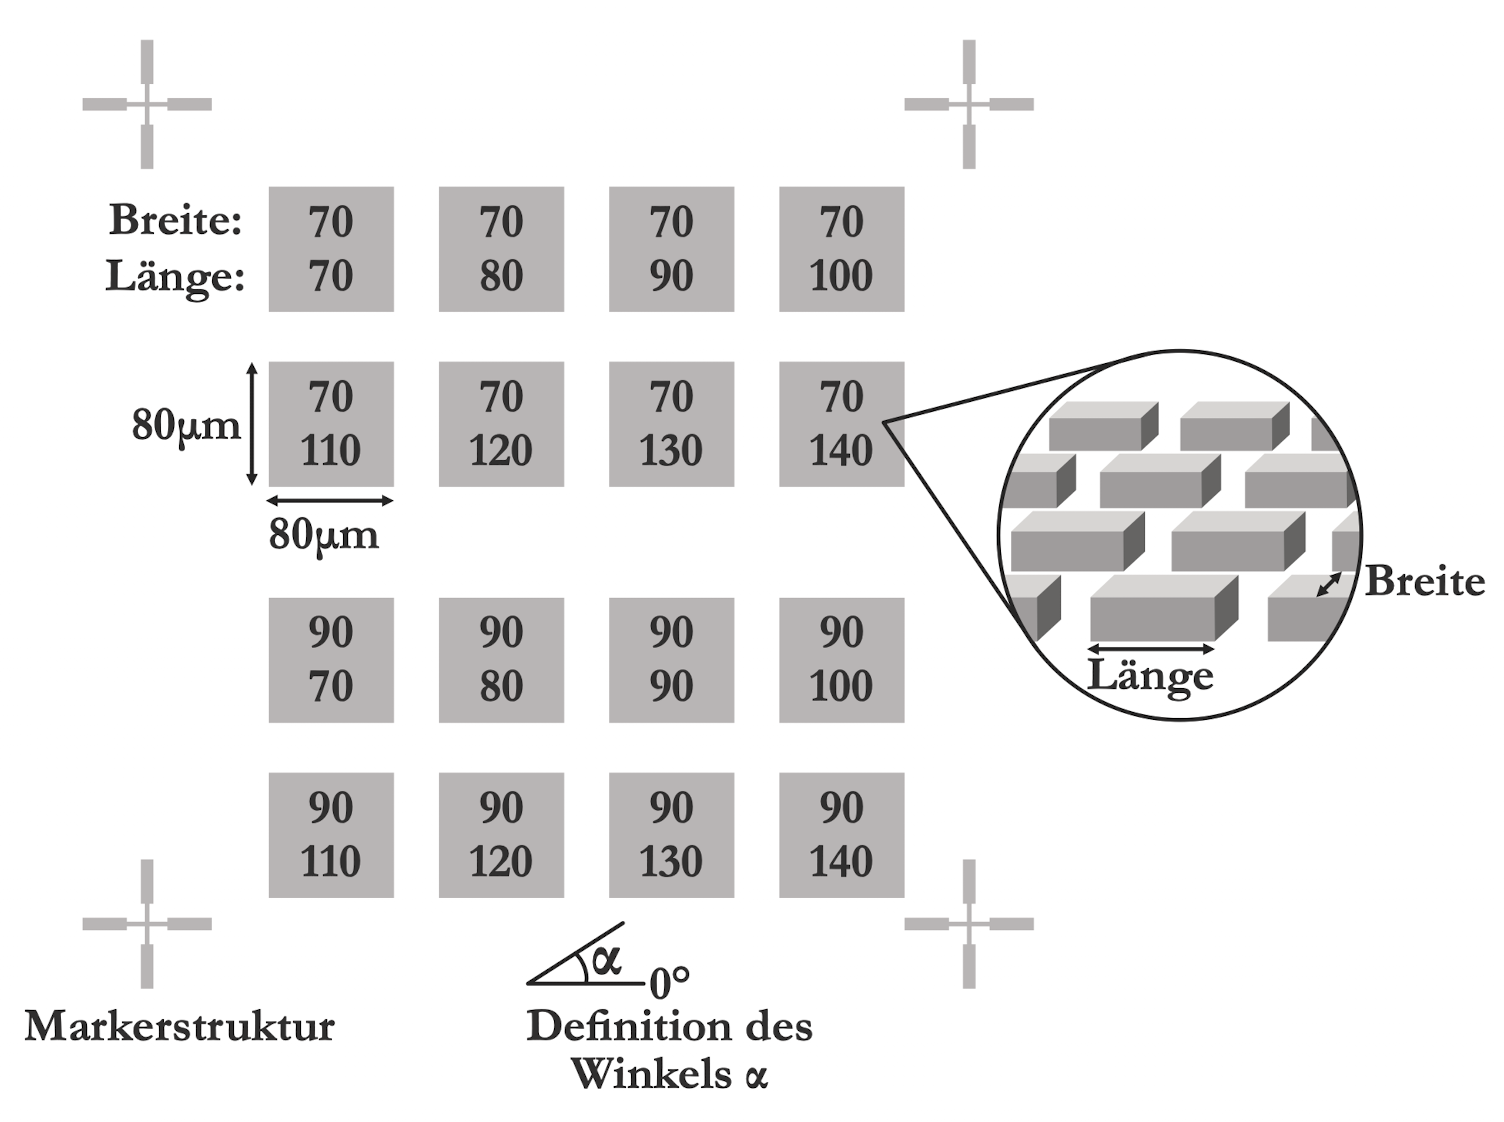
\includegraphics[width = \textwidth]{Bilder/Nanorods.png}
    \captionof{figure}{
        Übersichtsplan der verwendeten Probe. Die gesamte Probenstruktur befindet sich mehrmals auf einem Glassubstrat. Die Struktur selbst besteht aus Markern und 16 Feldern, die jeweils tausende Nanorod gleicher Dimensionen enthalten. Die Breite und Länge der Partikel in Nanometern sind auf den Feldern eingetragen. Das Inset zeigt die Vergrößerung eines einzelnen Probenfelds, wodurch die Orientierung der langen Achse der Rods und die Definition von Breite und Länge erkennbar ist. Der Winkel $\alpha$ ist unter dem Übersichtsplan definiert. Eine Polarisation von $\alpha = 0^\circ$ führt damit zu einer Anregung entlang der langen Achse der Rods. \cite{Anleitung}
    }
    \label{fig:nanorods}
\end{center}

In diesem Versuchsteil wurden mehrere Struktuten mit unterschiedlicher Nanorods (bestehend aus Silber) mit einer Breite $B$ von 70\,nm und 90\,nm und variabler Länge $L$ untersucht. Abbildung \ref{fig:nanorods} zeigt hierbei den Übersichtsplan der Probe, mit dem Parameter der Rods in den einzelnenFelder. Jedes Feld hat eine Größe von 80$\times$80\,$\mu$m und beinhaltet tausende identische Nanorods, womit das Streuspektrim aller Rods auf einem Feld gemessen werden kann. Der Winkel $\alpha$ gibt folgenden die Richtung der Polarisation an, wobei $\alpha = 0^\circ$ die Länge der Rods anregt und $\alpha = 90^\circ$ die Breite der Rods. \cite{Anleitung}
\bigskip

Es wurden einerseites die Spektren der Nanorods mit Intensität $I_\mathrm{N}$ als auch ein Dunkelspektrum $I_\mathrm{D}$ und ein Referenzspektrum $I_\mathrm{R}$ am Anfang und am Ende der Messung aufgenommen. Da in beiden Messungen das Dunkelspektrum mitgemessen wurde, wird dieses in der weiteren Rechnung nicht mehr beachtet (siehe auch Kapitel \ref{sub:korrigiertesSignal}). Um ein korrigieres Dunkelfeldspektrum $I_\mathrm{C}$ zu erhalten wird folgende Formel angewendet
\begin{gather}
    I_\mathrm{C} = \frac{I_\mathrm{N}}{\langle I_\mathrm{R} \rangle} ~,
\end{gather}
wobei $\langle I_\mathrm{R} \rangle$ der Mittelwert zwischen dem Referenzspektrum am Anfang und am Ende der Messung ist. Das korrigierte Dunkelfeldspektrum $I_\mathrm{C}$ (Einheit a.u. = arb. units) wurde in Abb. \ref{fig:spektrum} in Abhängigkeit der Wellenlänge $\lambda$ (Einheit nm) dargestellt. Dabei lässt sich für unpolarisiertes und polarisiertes Licht ($\alpha = 0^\circ$) erkennen, dass für zunehmende Rodlänge die Intensität $I_\mathrm{C}$ abnimmt. Für $\alpha = 90^\circ$ Polarisation ist dieser Effekt nur bei einer Rodbreite von 70\,nm zu erkennen, wobei hier zwei Maxima beobachtet werden können, welche selbst konstant sind für gewisse Rodlängen. Für eine Rodbreite von 90\,nm ist die Intensität unabhängig von der Rodlänge. Da erwartet wurde, dass sich die Intensität für eine Polarisation von $\alpha = 90^\circ$ nicht ändern sollte, lässt sich vermuten, dass bei der Messung von der Rodbreite 70\,nm ein Messfehler enstanden ist. Wieterhin lässt sich erkennen dass die Polarisation einen Einfluss auf die Position der Maxima hat, da für $\alpha = 90^\circ$ Polarisation die Maxima alle untereinander liegen und für $\alpha = 0^\circ$ Polarisation die Maxima verschoben sind für unterschiedliche Rodlängen $L$. Dieses Verhalten deckt sich auch mit der Literatur \citenum{Anleitung} und der Erklärung für das Verhalten der transversalen Moden ($\alpha = 90^\circ$) und longitudinalen Mode ($\alpha = 0^\circ$). Das unpolarisierte Spektrum zeigt dafür Charakteristiken der transversalen und longitudinalen Mode, was deutlich zu sehen ist an den lokalen Maxima des unpolarisierten Spektrums.  
\bigskip

Im nächsten Schritt wird durch einen Gauss-Fit die Wellenlänge der Maxima der Dunkelfeldspektren $\tilde{\lambda}$ bestimmt. Die berechenten Werte können in Tabelle \ref{tab:nanorods} gefunden werden und zeigen numerisch die Abhängigkeit der Position der Maxima in Bezug auf die Polarisationsrichtung. Die bestimmten Wellenlängen werden dann dafür benutzt, um die effektive Längenänderung $\Delta L$ der Rods und den effektive Berechungsindex der Fabry-Perot Moden in den Pratikel $n_\mathrm{eff}$ zu bestimmen. Dafür wird eine linearer Fit durch die Messwerte der $\alpha = 0^\circ$ Polarisation durchgeführt. Es wird folgende lineare Korrelation erwartet
\begin{gather}
    m\lambda = 2 (L(m) + \Delta L)n_\mathrm{eff}~,
\end{gather}
mit der Resonatorlänge $L(m) + \Delta L$. \cite{Anleitung} Beachtet man nur die Grundmode mit $m = 1$ erhält man
\begin{gather}
    \lambda(L) = 2 ( L + \Delta L) n_\mathrm{eff}~.
    \label{eq:effBrechung}
\end{gather}
Der lineare Fit wurde in Abb. \ref{fig:linFit} dargestellt, wobei die Messwerte für $L = 70$, 80, 130 und 140\,nm für $B = 70\,\mathrm{nm}$ und $L = 130$ und 140\,nm für $B = 90\,\mathrm{nm}$ ausgeschlossen wurden, weil sie nicht den Erwartungen entsprechen. 

Der Fit hat hierbei folgende Form
\begin{gather}
    \tilde{\lambda}^{\alpha = 0^\circ} = M \cdot L + \tilde{\lambda}^{\alpha = 0^\circ}_0~,
    \label{eq:fit}
\end{gather}
wobei $M$ die Steigung der Gerade ist und $\tilde{\lambda}^{\alpha = 0^\circ}_0$ der Achsenabschnitt. In Abb. \ref{fig:linFit} ist gut zu sehen, dass beide Fits in etwa die gleiche Gerade sind, was erwartet war, da $n_\mathrm{eff}$ und $\Delta L$ nicht von der Rodlänge $L$ abhängen sollte. Mittelung über die ermittelten Werte für unterschiedliche Rodbreiten $B$ ergibt
\begin{gather*}
    M = 2,2 \pm 0,2 \qquad \mathrm{und} \qquad \tilde{\lambda}^{\alpha = 0^\circ}_0 = (478 \pm 23)\,\mathrm{nm}~.
\end{gather*}
Vergleicht man nun Gleichung (\ref{eq:effBrechung}) und (\ref{eq:fit}) miteinander, findet man
\begin{gather}
    n_\mathrm{eff} = \frac{M}{2} \qquad \mathrm{und} \qquad \Delta L = \frac{\tilde{\lambda}^{\alpha = 0^\circ}_0}{M}~,
\end{gather}
was folgende Werte berechnen lässt
\begin{gather*}
    \boxed{n_\mathrm{eff} = 1,1 \pm 0,1 \qquad \Delta L = (218 \pm 22)\,\mathrm{nm}}~.
\end{gather*}
Der Wert $n_\mathrm{eff}$ liegt in der Erwartung, wenn man berücksichtigt, dass  $n_\mathrm{eff} = 1,4$ eine vernünftige Wahl für Partikel mit Wasser/Luft Grenzschicht ist \cite{Anleitung}. Das Ergebnis für die effektive Längenänderung $\Delta L$ liegen auch in den Erwartung der Literatur \citenum{Chen2013}, da das plasmonische elektrische Feld außerhalb eines Plasmons nicht die 100\,nm überschreitet, was in etwa in unserem Fall in etwa $\Delta L /2$ entsprechen würde.  
\newpage

\begin{center}
    \captionsetup{type = figure}
    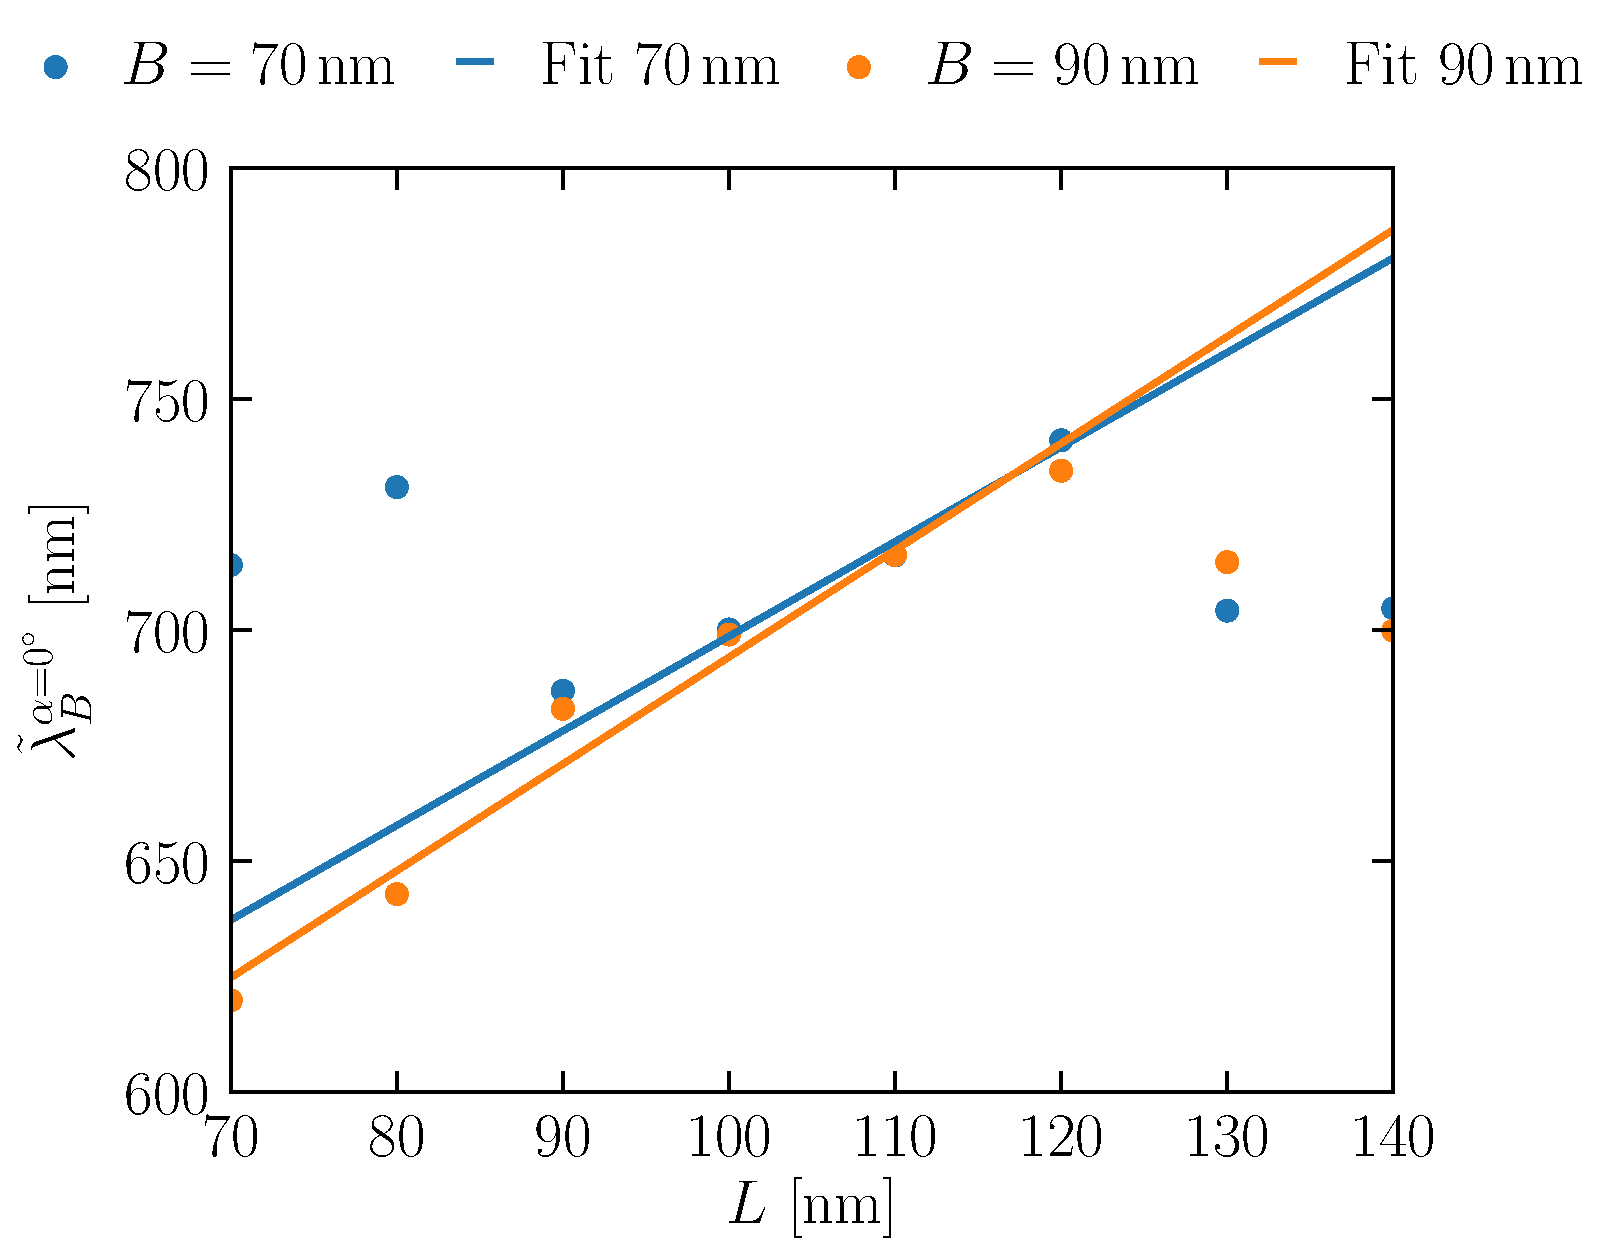
\includegraphics[width = 0.69\textwidth]{Bilder/Auswertung/3.2/Wavelength_Fit_Gruppe2.pdf}
    \captionof{figure}{
        Linearer Fit der Wellenlängen der Maxima im Dunkelfeldspektrum $\tilde{\lambda}$ für die Polarisation $\alpha = 0^\circ$ in abhängig der Rodlänge $L$ und Rodbreite $B$.
    }
    \label{fig:linFit}
\end{center}

\begin{center}
    \captionsetup{type = table}
    \begin{tabular}{r | c c c}
        $L$/nm & $\tilde{\lambda}^\mathrm{unpol}_{70}$/nm & $\tilde{\lambda}^\mathrm{\alpha = 0^\circ}_{70}$/nm & $\tilde{\lambda}^\mathrm{\alpha = 90^\circ}_{70}$/nm \\\hline
        70  & 704,97 $\pm$ 0,30 & 714,14 $\pm$ 0,25 & 664,06 $\pm$ 0,09 \\
        80  & 711,90 $\pm$ 0,45 & 731,00 $\pm$ 0,35 & 659,14 $\pm$ 0,10 \\
        90  & 670,03 $\pm$ 0,24 & 686,91 $\pm$ 0,28 & 651,89 $\pm$ 0,07 \\
        100 & 696,28 $\pm$ 0,15 & 700,19 $\pm$ 0,12 & 668,09 $\pm$ 0,06 \\
        110 & 711,12 $\pm$ 0,22 & 716,24 $\pm$ 0,15 & 668,05 $\pm$ 0,09 \\
        120 & 722,66 $\pm$ 0,47 & 741,14 $\pm$ 0,26 & 661,00 $\pm$ 0,11 \\
        130 & 669,37 $\pm$ 0,46 & 704,26 $\pm$ 0,34 & 653,20 $\pm$ 0,06 \\
        140 & 664,93 $\pm$ 0,26 & 704,78 $\pm$ 0,17 & 649,43 $\pm$ 0,05 \\
    \end{tabular}\\[0.5cm]
    \begin{tabular}{r | c c c}
        $L$/nm & $\tilde{\lambda}^\mathrm{unpol}_{90}$/nm & $\tilde{\lambda}^\mathrm{\alpha = 0^\circ}_{90}$/nm & $\tilde{\lambda}^\mathrm{\alpha = 90^\circ}_{90}$/nm \\\hline
        70  & 610,84 $\pm$ 1,64 & 619,92 $\pm$ 0,12 & 686,79 $\pm$ 0,29 \\
        80  & 653,88 $\pm$ 0,31 & 642,89 $\pm$ 0,09 & 678,25 $\pm$ 0,14 \\
        90  & 688,00 $\pm$ 0,06 & 683,02 $\pm$ 0,04 & 684,50 $\pm$ 0,06 \\
        100 & 703,85 $\pm$ 0,08 & 699,08 $\pm$ 0,07 & 690,43 $\pm$ 0,10 \\
        110 & 718,89 $\pm$ 0,13 & 716,34 $\pm$ 0,10 & 691,28 $\pm$ 0,09 \\
        120 & 735,59 $\pm$ 0,24 & 734,54 $\pm$ 0,15 & 687,75 $\pm$ 0,10 \\
        130 & 705,59 $\pm$ 0,14 & 714,76 $\pm$ 0,15 & 668,04 $\pm$ 0,09 \\
        140 & 689,79 $\pm$ 0,10 & 699,93 $\pm$ 0,15 & 664,27 $\pm$ 0,08 \\
    \end{tabular}
    \captionof{table}{
        Wellenlänge der Maxima des Dunkelfeldspektrum $\tilde{\lambda}$ für unpolarisiertes und polarisiertes ($\alpha = 0^\circ~;~90^\circ$) Licht für unterschiedliche Rodlängen $L$ und Rodbreiten $B$.
    }
    \label{tab:nanorods}
\end{center}

\newpage
\begin{sidewaysfigure}
    \centering
    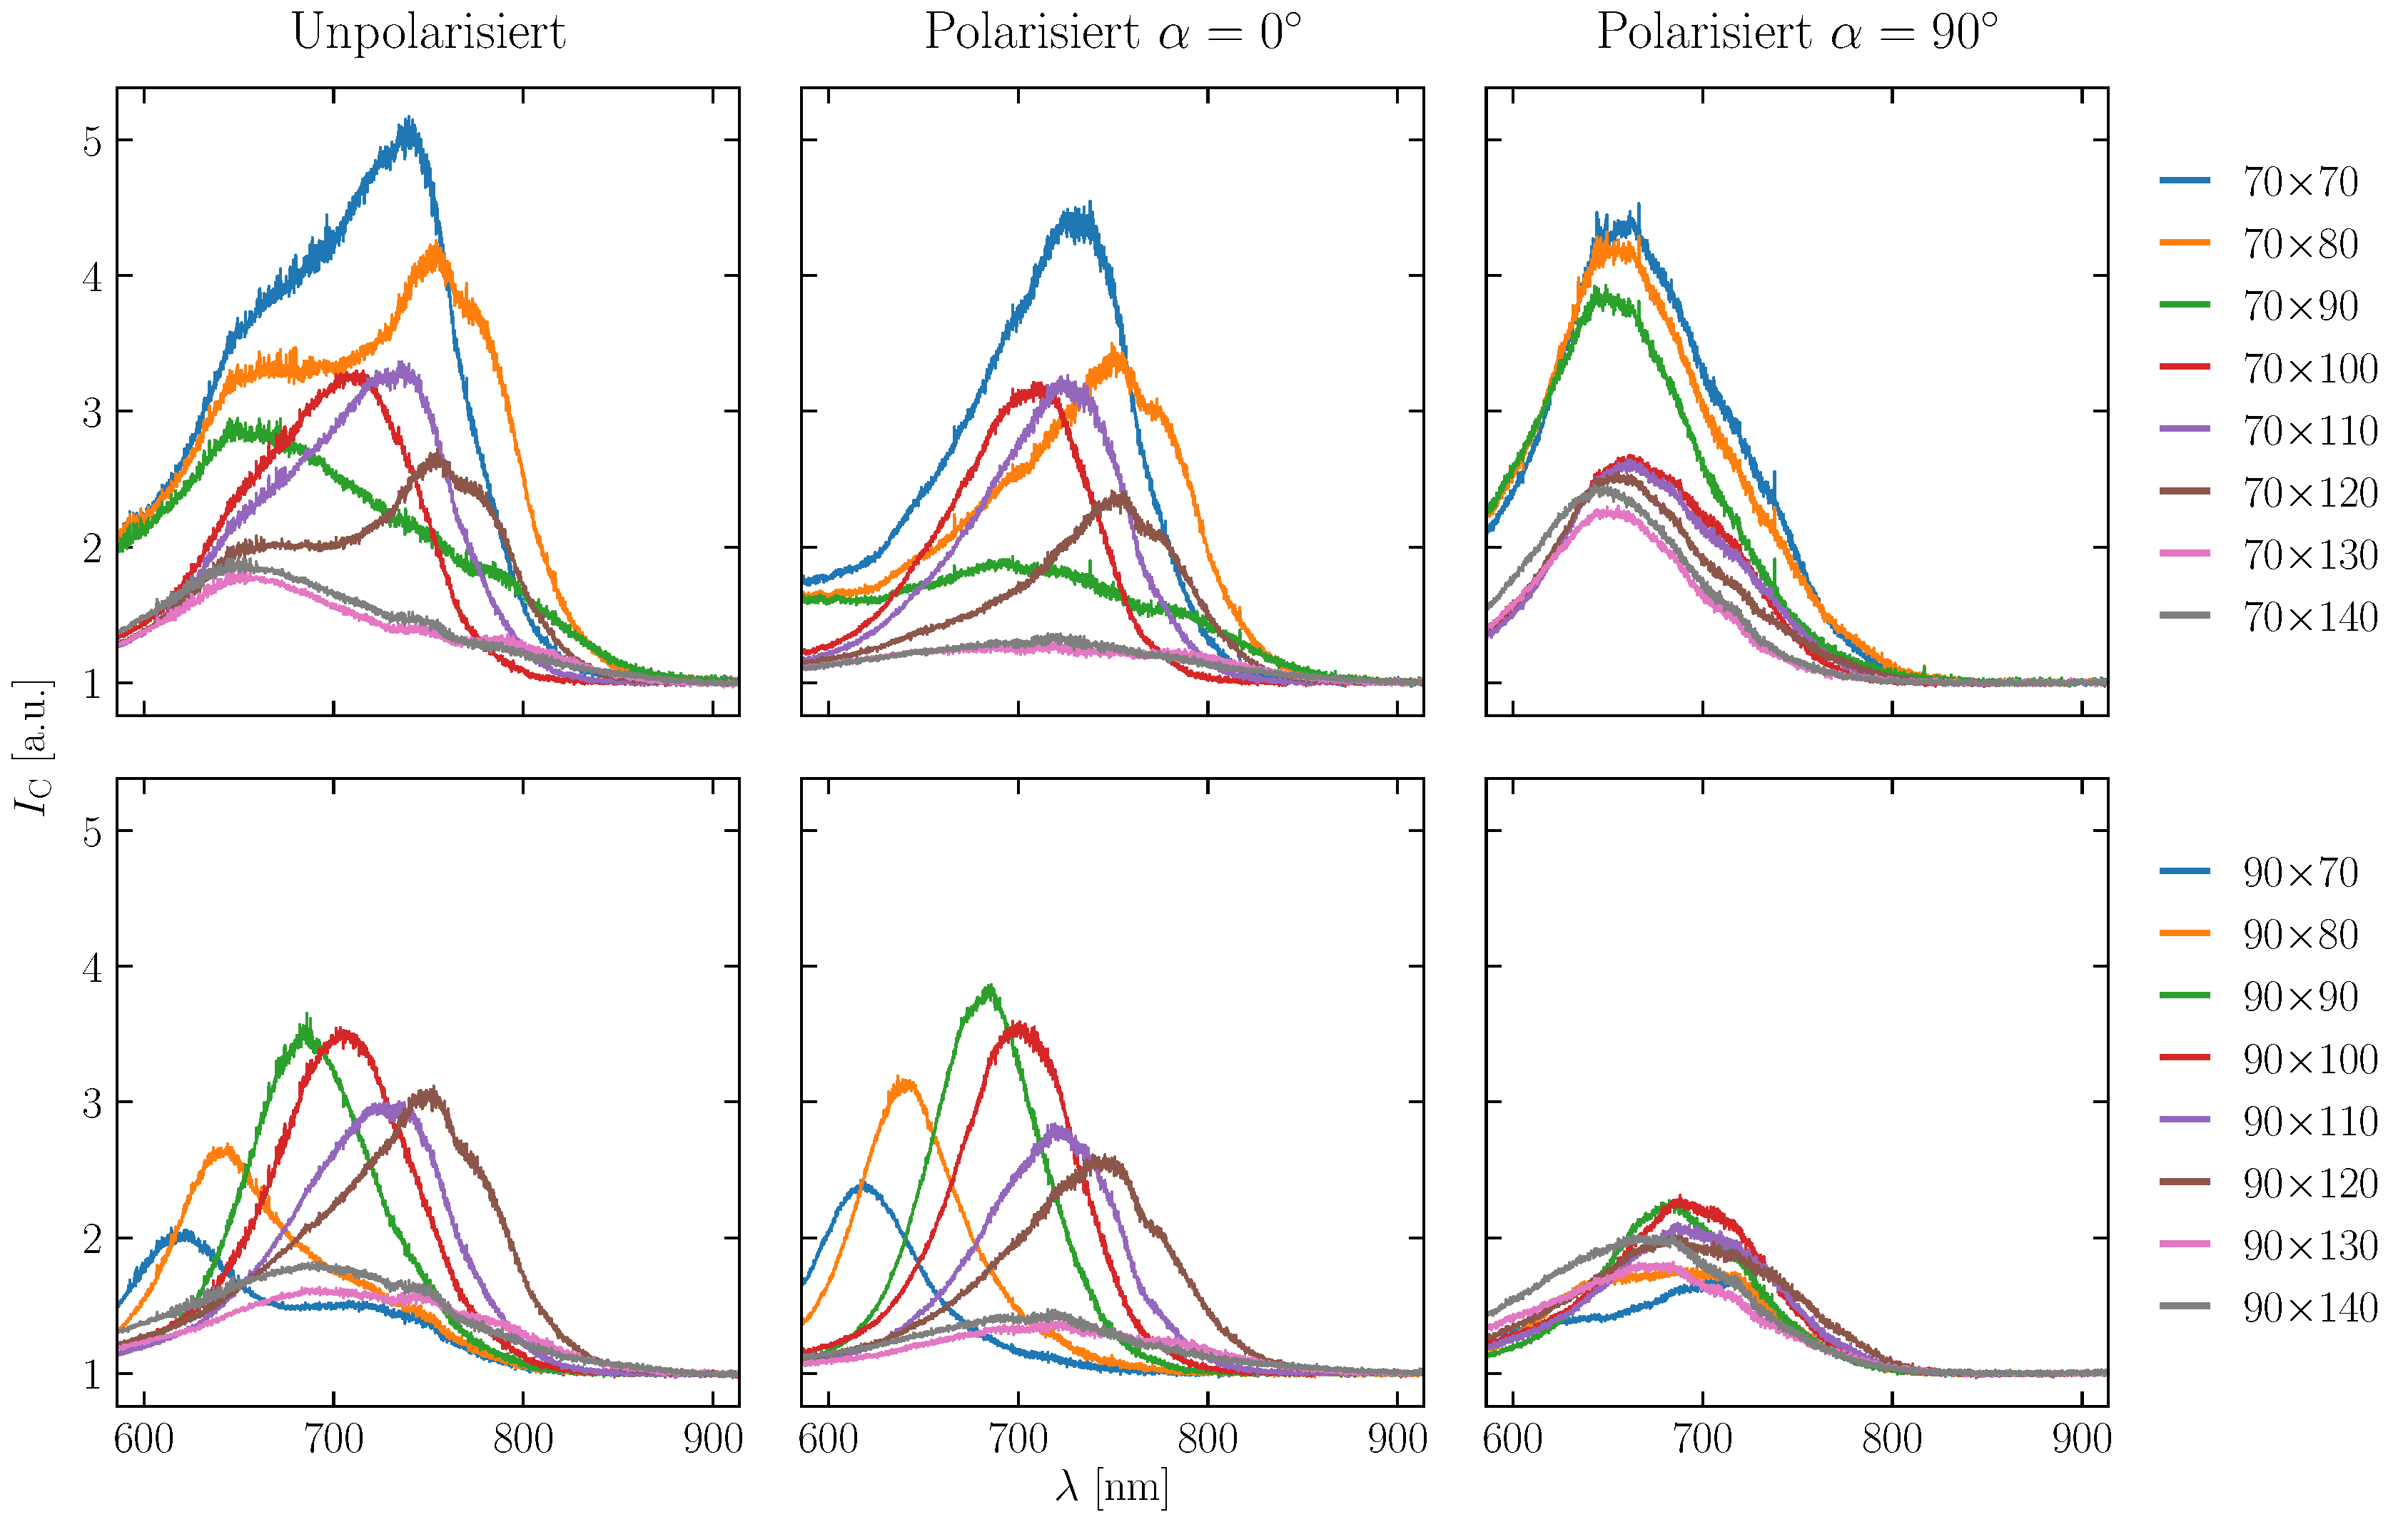
\includegraphics[width = \textheight]{Bilder/Auswertung/3.2/Spektren_Gruppe2.pdf}
    \caption{Korrigiertes Spektrum der Nanorodproben mit unpolarisierten und polarisierten ($\alpha = 0^\circ~;~90^\circ$) Lichtquelle. Die Rodlänge $L$ und die Rodbreite $B$ in Nanometer wurde mit Nomenklatur $B \times L$ dargestellt}
    \label{fig:spektrum}
\end{sidewaysfigure}